\chapter{Конструкторская часть}
В этом разделе приведены схемы алгоритмов линии конвейера и последовательного алгоритма обратной трассировки лучей, а также описаны возможности пользователя и приведена диаграмма взаимодействия конвейерных линий.

\section{Разработка алгоритмов}

На рисунках \ref{fig:follow}, \ref{fig:rtline} представлены схемы алгоритмов линии конвейера и последовательного алгоритма обратной трассировки лучей. Алгоритм обработки данных на линии конвейера представлен в универсальном виде, конкретизация выполняемой работы связана с блоком предопределённого процесса Action.

\begin{figure}[H]
	\centering
	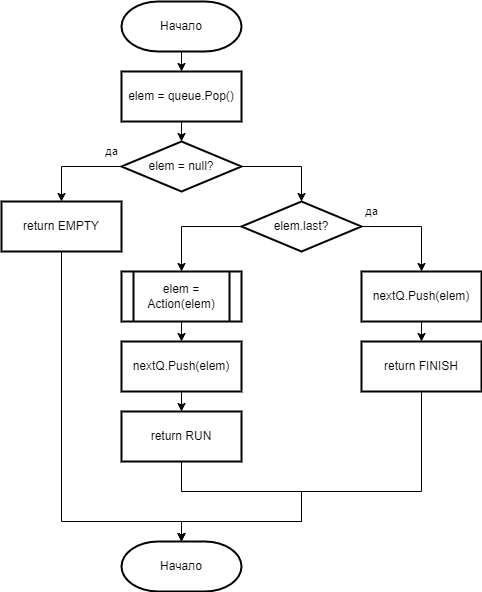
\includegraphics{inc/img/rtline}
	\caption{Схема алгоритма линии конвейера}
	\label{fig:rtline}
\end{figure}

\captionsetup{justification=centering,singlelinecheck=true}
\begin{figure}[H]
	\centering
	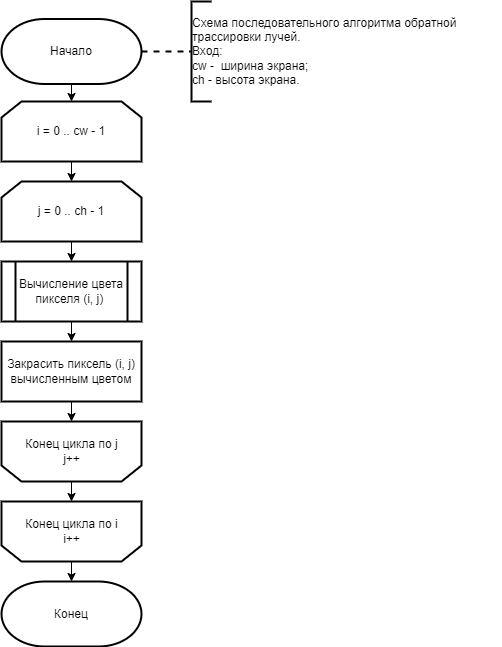
\includegraphics[width=0.7\linewidth]{inc/img/follow}
	\caption{Схема последовательного алгоритма обратной трассировки лучей}
	\label{fig:follow}
\end{figure}

\section{Возможности пользователя}

В списке приведены описания пунктов меню.

\begin{enumerate}
	\item Пользователь вводит количество частиц, размер частиц, время симуляции.
	Программа выводит сгенерированное изображение на экран.
	\item Программа выводит таблицу с временами выполнения реализаций алгоритма обратной трассировки лучей при разном количестве заявок.
	\item Программа пишет лог обработки заявок в файл.
	\item Программа выводит таблицу с временами выполнения реализаций алгоритма обратной трассировки лучей при разном количестве объектов.
\end{enumerate} 

\section{Диаграмма последовательности взаимодействия конвейерных линий}

На рисунке \ref{fig:conveyor} представлена диаграмма последовательности взаимодействия конвейерных линий.
\begin{figure}[H]
	\centering
	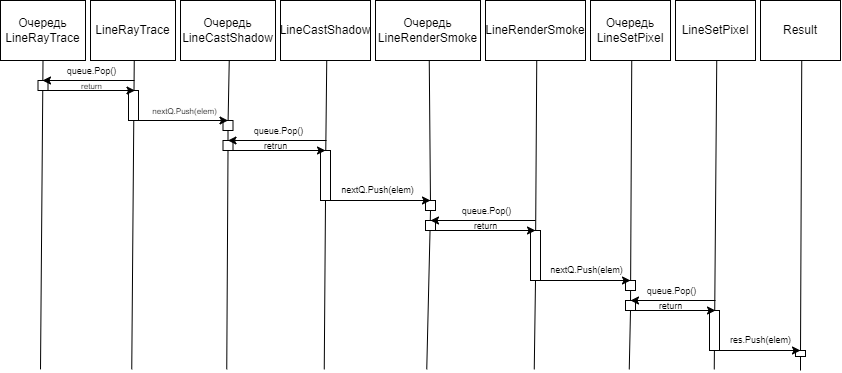
\includegraphics[width=1\linewidth]{inc/img/conveyor}
	\caption{Диаграмма взаимодействия конвейерных линий}
	\label{fig:conveyor}
\end{figure}



\section*{Вывод}

Были приведены схемы алгоритмов линии конвейера и последовательного алгоритма обратной трассировки лучей, а также описаны возможности пользователя и приведена диаграмма последовательности взаимодействия конвейерных линий.


